\documentclass[11pt,a4paper]{article}
\usepackage[margin=2.2cm]{geometry}
\usepackage{graphicx}
\usepackage{booktabs}
\usepackage{caption}
\usepackage{subcaption}
\usepackage{float}
\usepackage{amsmath}
\usepackage{xcolor}
\usepackage{listings}
\usepackage[hidelinks]{hyperref}
\usepackage{enumitem}
\graphicspath{{../plots/}}
\setlength{\parskip}{4pt}
\captionsetup{font=small,labelfont=bf}

\lstset{basicstyle=\ttfamily\footnotesize,breaklines=true,frame=single,columns=fullflexible,keepspaces=true}

% ------------------------------------------------------------------
% TEAM
% ------------------------------------------------------------------
\newcommand{\teamtable}{%
\begin{tabular}{ll}
\toprule
Name & Roll number \\
\midrule
Pranav & 24B1074 \\
Atharva & 24B0996 \\
Divyaansh & 24B0981 \\
Sufiyan & 24B0935 \\
\bottomrule
\end{tabular}}

\title{\textbf{CS683 PA1, Task 1: 2D Convolution, the Dhurandhar Way}\\[4pt]
\large Loop reordering, unrolling, cache tiling, SIMD, and their combination}
\author{\teamtable}
\date{Autumn 2026}

\begin{document}
\maketitle

\section{Setup and methodology}

\paragraph{Machine.} All numbers in this report come from one Intel Core i7-13700HX (Raptor Lake, hybrid). We pinned every run to CPU~0, a P-core, with \texttt{taskset} and set the frequency governor to \texttt{performance}. \texttt{lscpu -C} reports L1-D 48\,KB, 12-way, 64\,B lines; L2 1.25\,MB per P-core; L3 30\,MB shared. The consumer Raptor Lake parts have AVX-512 fused off, so the SIMD experiments use 128-bit (xmm) and 256-bit (ymm) registers only.

\paragraph{Build.} We used the pinned flags from the provided \texttt{Makefile} for every stage and did not change them: \texttt{-std=c++17 -O2 -fno-tree-vectorize -mavx2 -mfma}. Auto-vectorisation is off, so any vector code in the binaries is ours. The provided harness (\texttt{main.cpp}) takes the median of 7 timed repetitions after 2 warm-ups, checks every stage against \texttt{conv\_naive} (max abs error $<10^{-3}$), and reports speedup as $t_{\text{naive}}/t_{\text{stage}}$ on the same input.

\paragraph{Profiling.} Counters come from \texttt{perf stat} (\texttt{L1-dcache-load-misses}, \texttt{instructions}). The harness always runs the naive reference before the stage under test (once for the check, then 2 warm-ups and 7 reps), so we obtained per-call counts by subtraction: a naive-only run gives the cost of the reference calls, and we subtract that from the run that also contains the stage. MPKI is $10^3 \times$ L1-D misses divided by the instructions of the stage being measured.

\paragraph{Correctness.} All five stages pass the harness smoke tests. We also checked them on ragged shapes: $100\times8$ with $K=7$, $33\times16$ with $K=1$, $257\times520$ with $K=9$, $1\times8$ with $K=5$, and $2050\times2056$ with $K=3$. No stage assumes power-of-two sizes. Tile loops clamp at the image edge and the SIMD stages keep a scalar tail.

\paragraph{How the stages relate to the naive code.} The naive loop nest is \texttt{oy, ox, ky, kx}: each output pixel is finished before the next one starts, from a $K\times K$ window. That order already has good locality, since the window slides by one column, so tiling has nothing to fix in it. The reordered nest (\texttt{ky, kx, oy, ox}) is the form where the inner loop becomes a unit-stride sweep over a whole output row, and that sweep is what unrolling, tiling and SIMD each act on. \texttt{conv\_unroll}, \texttt{conv\_tile} and \texttt{conv\_simd} therefore each start from the naive arithmetic with only that reorder applied and add exactly one technique, so the speedup of each file measures that technique. \texttt{conv\_optimized} is a different design that combines them (Section~\ref{sec:1d}).

\section{Task 1A: loop reordering and unrolling}

\subsection{What we changed and why}

Reordering (\texttt{conv\_reorder.cpp}). The kernel loops move outermost, the output is zeroed once, and for every tap $(k_y,k_x)$ the whole image is swept with \texttt{out[oy][ox] += in[oy+ky][ox+kx] * w}. The motivation is that the naive inner loop over $k_x$ runs only 3 or 5 times, so most of its cost is loop overhead, index arithmetic and reloading the weight. After the reorder the innermost loop is $W$ iterations of one multiply-accumulate with unit stride on both \texttt{in} and \texttt{out}, which is what the hardware prefetchers and, later, the vector unit want. The weight $w$ is loop-invariant and stays in a register.

Unrolling (\texttt{conv\_unroll.cpp}). We unroll the column loop by 8. The harness guarantees $W$ is a multiple of 8, and 8 floats is one AVX register, which keeps this stage in step with the SIMD stage later. The 8 partial sums live in a local array \texttt{a[8]} that the compiler keeps in registers across the whole $k_x$ loop; the running value is read from \texttt{out} once per $k_y$ and written back once. We had three things in mind. The 8 accumulators are independent, so a single accumulator's latency chain is broken and the core can overlap 8 multiply-adds. Loop control and indexing are amortised over 8 pixels. And \texttt{out} traffic drops from $K^2$ read-modify-writes per pixel to $K$, one per $k_y$, because the $k_x$ loop accumulates in registers.

\subsection{Effectiveness and the metric}

We measure effectiveness as wall-clock speedup over \texttt{conv\_naive} on the same input, because that is what a caller of the routine sees and what the harness grades. GFLOP/s appears alongside it; the FLOP count is identical for every stage, so it is the same information on an absolute scale. Instruction count and MPKI appear in later sections to explain results, not as the target.

\begin{table}[H]
\centering\small
\caption{Reorder and unroll, speedup over naive (median of 7). Data: \texttt{task1d\_sections234\_fixed.txt}.}
\begin{tabular}{lrrrrrr}
\toprule
$K=3$, $H=W$ & 256 & 512 & 1024 & 2048 & 4096 \\
\midrule
naive time (ms)      & 0.274 & 1.161 & 3.936 & 16.69 & 58.35 \\
reorder speedup      & 1.19$\times$ & 1.51$\times$ & 1.57$\times$ & 1.14$\times$ & 0.78$\times$ \\
unroll speedup       & 3.06$\times$ & 3.28$\times$ & 3.42$\times$ & 3.30$\times$ & 2.44$\times$ \\
\midrule
$K=5$, $H=W$ & 256 & 512 & 1024 & 2048 & \\
\midrule
reorder speedup      & 1.84$\times$ & 1.85$\times$ & 1.37$\times$ & 1.33$\times$ & \\
unroll speedup       & 4.13$\times$ & 4.37$\times$ & 3.31$\times$ & 4.21$\times$ & \\
\bottomrule
\end{tabular}
\end{table}

Reordering on its own is a small win that depends on size, and at 4096 it is a loss. While the image fits in L2/L3 (up to $2048\times2048$, a 16\,MB output) the simpler inner loop gains 1.1 to 1.6$\times$. At $4096^2$ the output is 64\,MB, more than L3, and the reordered code now makes $K^2=9$ full passes over \texttt{out} and \texttt{in} from DRAM where naive makes one. It drops to 0.78$\times$. The README warns about exactly this, and it is the memory-bound behaviour that tiling (1B) exists to remove.

Unrolling is a steady $\approx3\times$. Its three sources do not depend on cache behaviour: register accumulation across $k_x$ (fewer \texttt{out} loads and stores), 8 independent dependency chains, and amortised loop overhead. It stays nearly flat across sizes and keeps most of its gain at 4096, where reorder collapses, because it makes only $K$ passes over \texttt{out} instead of $K^2$. At $K=5$ there is more arithmetic per pixel relative to memory traffic and the gain rises to as much as 4.4$\times$.

\section{Task 1B: cache tiling}

\subsection{Baseline profile}

The L1 data cache is 48\,KB, 12-way set associative, 64\,B lines, 64 sets. For the naive convolution at $K=3$ the L1-D MPKI is very low, between 0.13 and 0.31 across sizes 512 to 8192 (Table~\ref{tab:1b-size}). Part of that is genuine reuse of the sliding window from L1. Most of it is the denominator: the naive kernel executes a very large number of instructions per pixel ($K^2$ multiply-adds, each with its own index arithmetic and weight reload). The reordered version does the same arithmetic in about 12$\times$ fewer instructions and shows what streaming the whole image $K^2$ times actually costs: 6 to 8 MPKI.

\subsection{Tiled implementation and tile sweep}

\texttt{conv\_tile.cpp} blocks the output into $\text{TH}\times\text{TW}$ tiles. Inside each tile it runs the reordered nest (\texttt{ky, kx, oy, ox}), so all $K^2$ taps are applied to the tile while its $(\text{TH}+K-1)\times(\text{TW}+K-1)$ input patch and $\text{TH}\times\text{TW}$ output block are still in cache. Tile edges are clamped, so any $H$ and $W$ work. TH and TW are compile-time constants (\texttt{-DTH=... -DTW=...}), so the sweep recompiles instead of editing the file.

\begin{figure}[H]
\centering
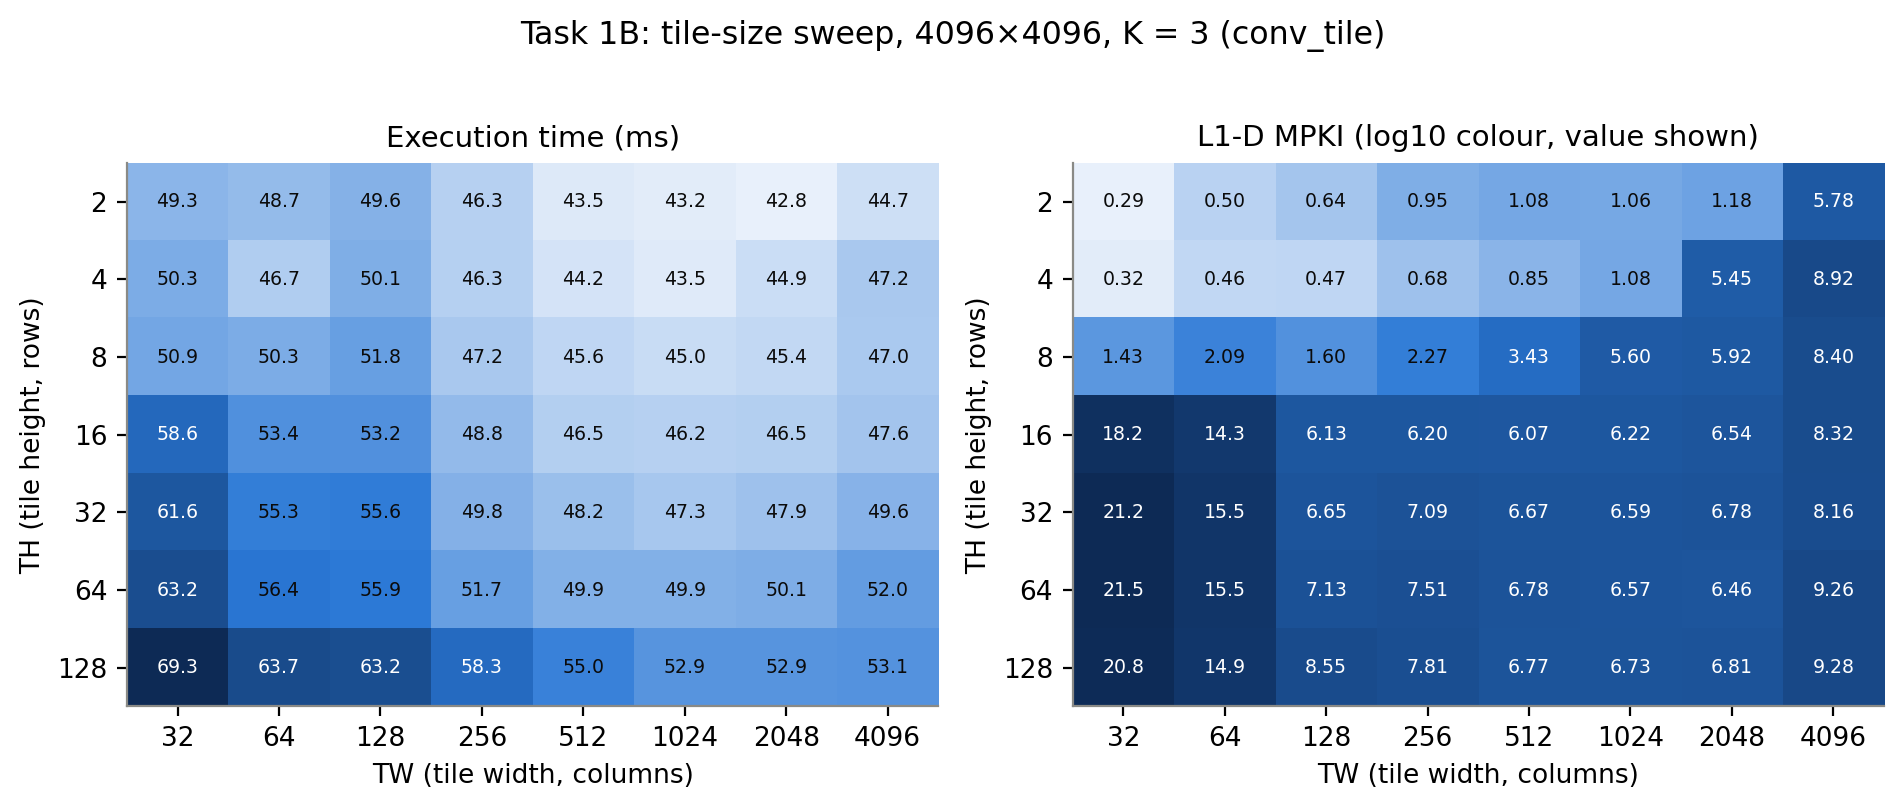
\includegraphics[width=\textwidth]{task1_tile_sweep.png}
\caption{Execution time (left) and L1-D MPKI (right) of \texttt{conv\_tile} over a $7\times8$ grid of tile shapes, $4096\times4096$, $K=3$. Data: \texttt{task1b\_full.txt} Section~2.}
\label{fig:tilesweep}
\end{figure}

Figure~\ref{fig:tilesweep} has three regions.

With TH $\le 4$ and TW $\le 1024$ the MPKI is low (0.3 to 1.1) and these are the fastest tiles (42.8 to 46.7\,ms). The tile's working set is roughly (TH+2)$\cdot$TW$\cdot$4\,B of input plus TH$\cdot$TW$\cdot$4\,B of output, 24\,KB at TH=4, TW=1024, which fits in L1 with room to spare.

At TW = 4096, the full width, MPKI jumps to 5.8 to 9.3. One row of input plus one of output at 4096 floats is already 32\,KB, and the $K^2$ passes over TH such rows no longer fit.

At TH $\ge 16$ the MPKI jumps to between 6 and 21 whatever TW is, even for tiny tiles: TH=16, TW=32 touches only 2.3\,KB of data yet shows 18 MPKI. Capacity cannot explain that. What does is the row stride. At 4096 the stride is 16\,KB, and the L1 set index comes from address bits 6 to 11, a 4\,KB period, so every row of \texttt{out} lands in the same 12-way set, and so do the padded \texttt{in} rows (stride 16,392\,B). Touching 16 output rows and 18 input rows of one tile column puts about 34 lines into a set with 12 ways, and the result is conflict misses. With TH $\le 8$ the per-set demand across the two arrays is at most about 18 lines and the aliasing is partly absorbed; at TH=4 it fits within 12 ways easily. This is the usual power-of-two-stride associativity problem, and it is why the fastest tiles here are short and wide rather than square.

Choice of tile. By execution time the optimum is the flat region TH=2 to 4, TW=1024 to 2048; five repeat runs at TH=2/TW=2048 and TH=4/TW=1024 land within 1\,ms of each other. By MPKI the optimum is TH=2, TW=32 (0.30), but it is 15\% slower, because very narrow tiles pay the $K^2$ loop-startup cost every 32 columns and hand the L2 streamer only 128\,B runs. We ship TH=4, TW=1024. It sits in the fastest group at every image size we tested (Table~\ref{tab:1b-size}), its 24\,KB working set leaves half of L1 free for the halo and \texttt{out}, and its MPKI of about 1 is 6 to 7$\times$ below the untiled reorder.

\subsection{MPKI and speedup versus matrix size}

\begin{table}[H]
\centering\footnotesize
\caption{L1-D MPKI and speedup over naive for the untiled and tiled kernels across image sizes, $K=3$. Data: \texttt{task1b\_full.txt} Section~4.}
\label{tab:1b-size}
\setlength{\tabcolsep}{3.5pt}\scriptsize
\begin{tabular}{l rrrrr rrrrr}
\toprule
& \multicolumn{5}{c}{L1-D MPKI} & \multicolumn{5}{c}{Speedup vs naive} \\
\cmidrule(lr){2-6}\cmidrule(lr){7-11}
$H=W$ & 512 & 1024 & 2048 & 4096 & 8192 & 512 & 1024 & 2048 & 4096 & 8192 \\
\midrule
naive                & 0.196 & 0.139 & 0.131 & 0.197 & 0.311 & 1.00 & 1.00 & 1.00 & 1.00 & 1.00 \\
reorder (untiled)    & 6.761 & 7.784 & 6.844 & 6.271 & 6.067 & 1.22 & 1.46 & 1.16 & 1.00 & 0.99 \\
tile TH=4, TW=64     & 0.376 & 0.446 & 0.433 & 0.405 & 0.393 & 1.44 & 1.57 & 1.45 & 1.44 & 1.48 \\
tile TH=4, TW=256    & 0.550 & 0.619 & 0.659 & 0.693 & 0.650 & 1.53 & 1.56 & 1.69 & 1.44 & 1.37 \\
tile TH=4, TW=1024   & 0.594 & 0.743 & 1.026 & 1.063 & 1.014 & 1.60 & 1.78 & 1.77 & 1.54 & 1.37 \\
tile TH=16, TW=512   & 5.536 & 5.466 & 5.856 & 6.150 & 6.638 & 1.91 & 1.45 & 1.58 & 1.42 & 1.49 \\
tile TH=32, TW=128   & 6.407 & 6.620 & 6.784 & 6.647 & 7.858 & 1.48 & 1.33 & 1.39 & 1.24 & 1.19 \\
\bottomrule
\end{tabular}
\end{table}

\begin{figure}[H]
\centering
\begin{subfigure}{0.52\textwidth}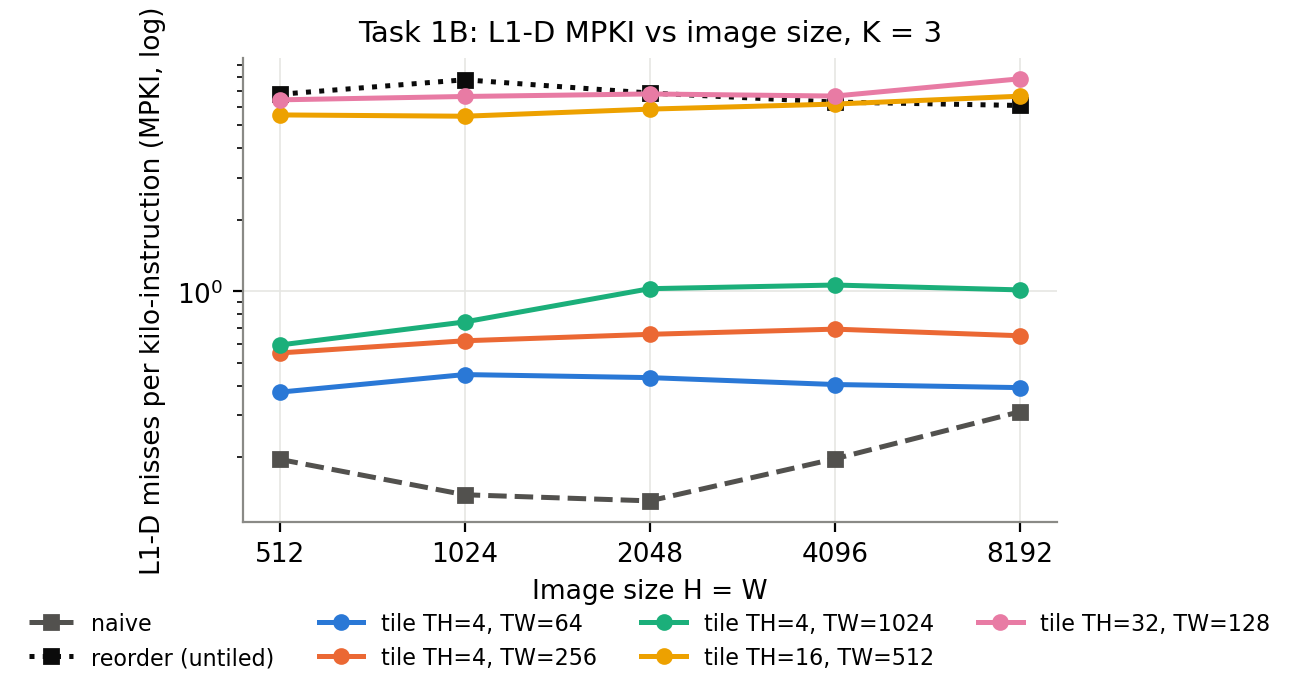
\includegraphics[width=\textwidth]{task1_mpki_vs_size.png}\end{subfigure}\hfill
\begin{subfigure}{0.46\textwidth}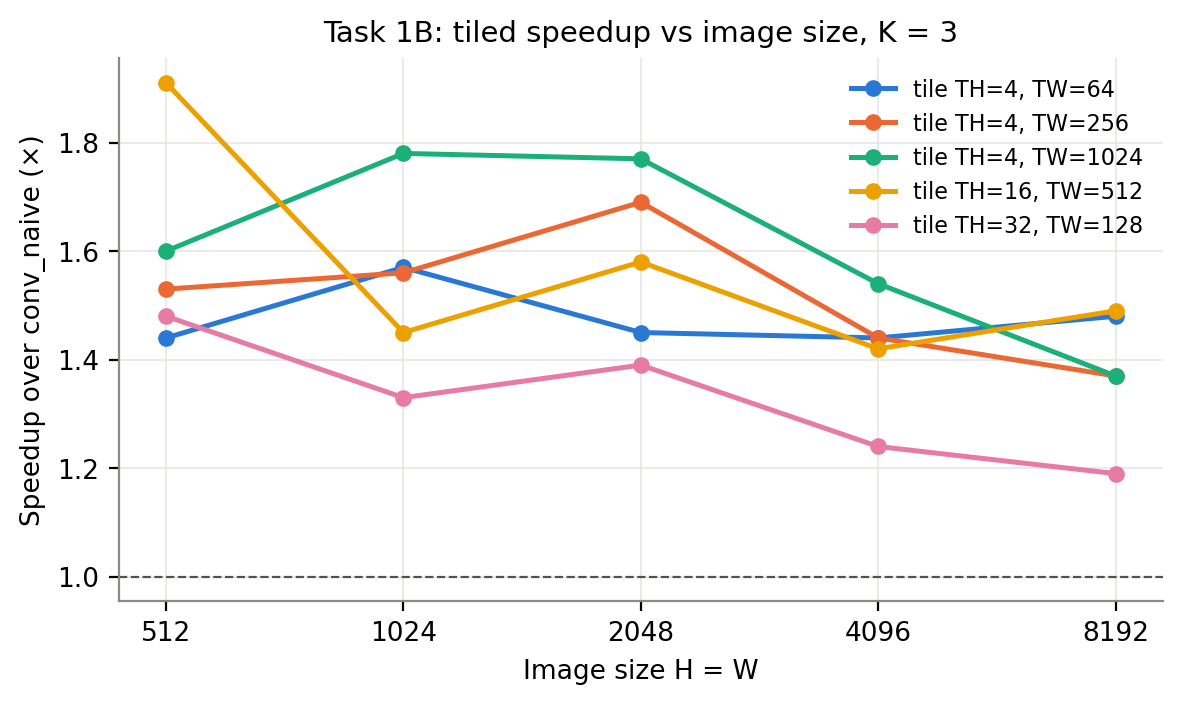
\includegraphics[width=\textwidth]{task1_tile_speedup_vs_size.png}\end{subfigure}
\caption{Left: L1-D MPKI versus image size for naive, untiled reorder and five tile shapes (log scale). Right: speedup of the tiled kernel over naive for the same tile shapes. $K=3$.}
\label{fig:1b}
\end{figure}

\subsection{Answers}

\textbf{Q1.} Measured directly, MPKI goes up from about 0.2 (naive) to 0.4 to 1.0 (tiled, TH=4). That is the denominator again. MPKI is per thousand instructions, and the naive kernel spends about 12$\times$ more instructions per pixel on loop control, indexing and weight reloads, so its misses per instruction look small even though it has no cache-reuse advantage over the tiled code. The comparison that shows what tiling does to the cache is reorder versus tile, which have the same instruction count: MPKI falls from 6 to 8 down to 0.4 to 1.0, a 7 to 17$\times$ reduction. Each tile's input patch and output block are read $K^2$ times from L1 instead of the whole image being streamed $K^2$ times from L2, L3 or DRAM.

\textbf{Q2.} For a fixed good tile (TH=4) the MPKI barely moves with image size: 0.38 to 0.45 at TW=64, 0.59 to 1.06 at TW=1024. That is what a working set bounded by the tile rather than by the image looks like; the cache sees the same 24\,KB problem whatever $H$ and $W$ are. MPKI grows with TW because longer rows mean fewer rows resident in L1, so the halo rows get fetched again more often. Across tile shapes the TH threshold from the sweep dominates: TH $\ge 16$ gives 5.5 to 7.9 MPKI at every size, no better than not tiling, because set conflicts rather than capacity decide the outcome. The naive kernel's own MPKI rises from 0.13 to 0.31 with size because at 8192 the $K$ input rows and the output row, 32\,KB each, no longer all fit in L1 together.

\textbf{Q3.} Yes. With TH=4, TW=1024 the tiled kernel is 1.37 to 1.78$\times$ faster than naive and 1.1 to 1.7$\times$ faster than the untiled reorder at every size. Tiling turns the $K^2$ image-wide streams into passes over L1-resident data, so the reorder's collapse at 4096 (0.78 to 1.00$\times$) disappears and the tiled speedup holds at 1.4 to 1.5$\times$ even with a 256\,MB output. The gain stops at about 1.7$\times$ because once the data comes from L1 the kernel is limited by scalar issue: every pixel-tap still costs a load, a multiply-add and a store of \texttt{out}. That is a compute-side limit, which tiling cannot touch, and it is the reason for 1C and 1D. One more observation: the speedup ranking and the MPKI ranking of tile shapes disagree. TW=64 has the fewest misses, TW=1024 the best time. An L1 miss that hits L2 costs about 14 cycles and is hidden by out-of-order execution and the L2 streamer when the run is long, so a lower MPKI is not worth $K^2$ extra loop restarts every 64 columns.

\section{Task 1C: SIMD}

\subsection{Implementation}

{\sloppy \texttt{conv\_simd.cpp} vectorises the reordered nest. For each tap the weight is broadcast once with \texttt{\_mm256\_set1\_ps}, and the row loop handles 8 output columns per iteration: an unaligned load of the input row (\texttt{\_mm256\_loadu\_ps} at \texttt{in+ox+kx}), an unaligned load of the current output, one \texttt{\_mm256\_fmadd\_ps}, and an unaligned store. A scalar tail covers $W \bmod 8$; the harness never takes it, but we kept it. The 128-bit variant is the same code with the \texttt{\_\_m128} type and the \texttt{\_mm\_*} intrinsics, selected at compile time with \texttt{-DSIMD\_W=128}. We checked both builds by disassembly: the 256-bit binary contains \texttt{ymm} FMAs, the 128-bit one contains none. AVX-512 is not available on this processor.\par}

\subsection{Instruction count and speedup}

\begin{table}[H]
\centering\footnotesize
\caption{Instructions retired per call (perf, subtracted) and speedup over naive for the SIMD kernel by width. Data: \texttt{task1c\_full.txt} Section~4.}
\label{tab:1c}
\begin{tabular}{l l rrr rr}
\toprule
$K$ & $H=W$ & naive instr. & SIMD-128 instr. & SIMD-256 instr. & red. 128 / 256 & speedup 128 / 256 \\
\midrule
3 & 1024 & $9.96\times10^{7}$ & $1.51\times10^{7}$ & $8.01\times10^{6}$ & 6.61 / 12.44 & 2.50 / 2.49 \\
3 & 2048 & $3.97\times10^{8}$ & $6.03\times10^{7}$ & $3.19\times10^{7}$ & 6.59 / 12.46 & 1.92 / 2.18 \\
3 & 4096 & $1.59\times10^{9}$ & $2.41\times10^{8}$ & $1.28\times10^{8}$ & 6.60 / 12.46 & 1.21 / 1.36 \\
3 & 8192 & $6.36\times10^{9}$ & $9.62\times10^{8}$ & $5.10\times10^{8}$ & 6.61 / 12.48 & 1.04 / 1.13 \\
5 & 1024 & $2.15\times10^{8}$ & $4.05\times10^{7}$ & $2.09\times10^{7}$ & 5.31 / 10.29 & 2.21 / 2.72 \\
5 & 2048 & $8.59\times10^{8}$ & $1.62\times10^{8}$ & $8.29\times10^{7}$ & 5.32 / 10.37 & 2.03 / 2.19 \\
5 & 4096 & $3.44\times10^{9}$ & $6.45\times10^{8}$ & $3.31\times10^{8}$ & 5.33 / 10.39 & 1.31 / 1.38 \\
5 & 8192 & $1.38\times10^{10}$ & $2.58\times10^{9}$ & $1.32\times10^{9}$ & 5.33 / 10.41 & 1.29 / 1.32 \\
\bottomrule
\end{tabular}
\end{table}

\begin{figure}[H]
\centering
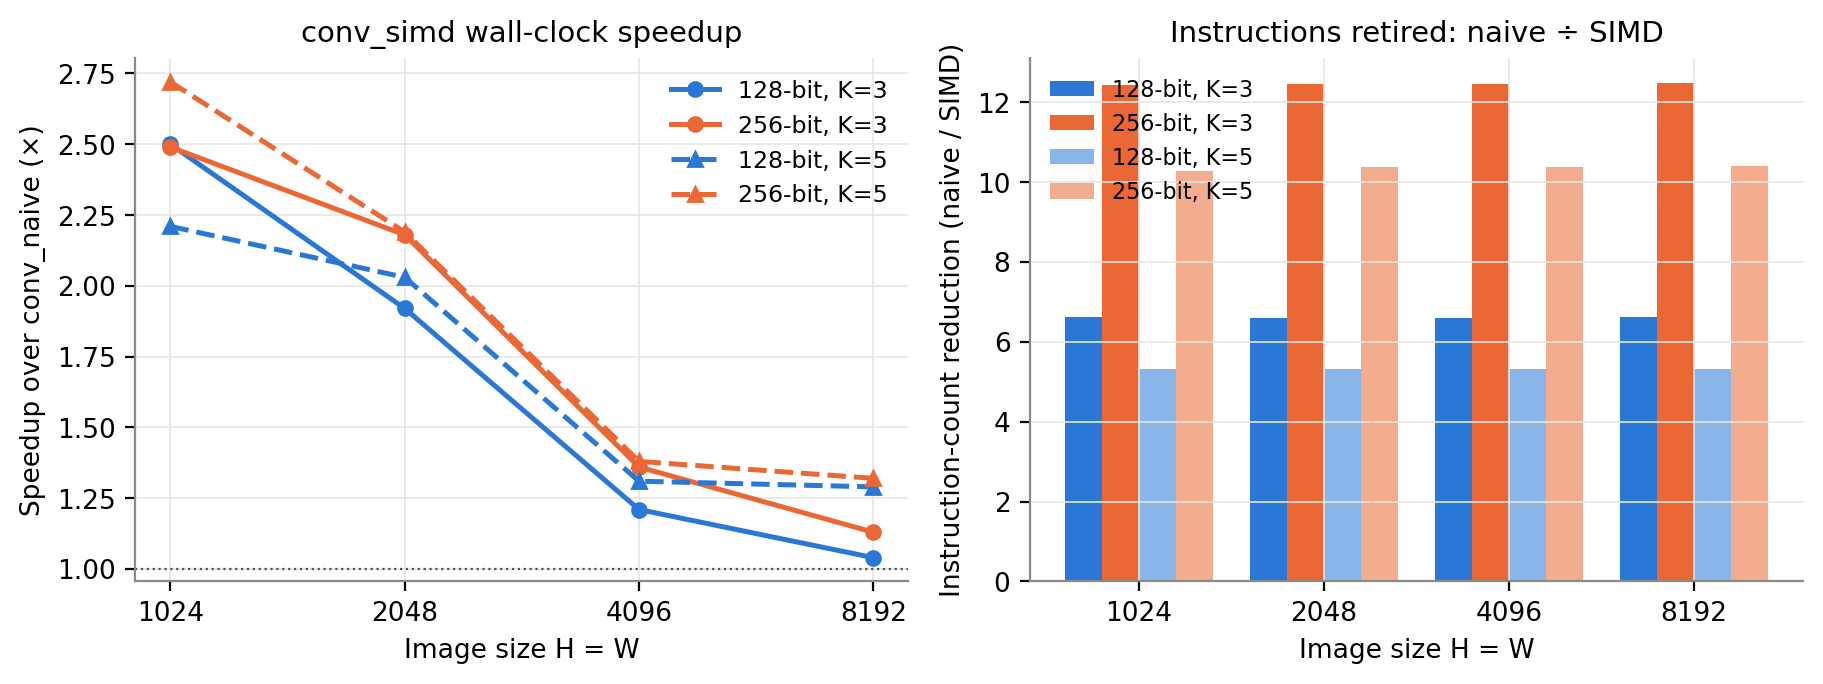
\includegraphics[width=\textwidth]{task1_simd_width.png}
\caption{Left: speedup of \texttt{conv\_simd} over naive versus image size for 128-bit and 256-bit builds. Right: instruction-count reduction factor. The 256 and 512 sizes run in well under a millisecond and were left out as too noisy.}
\end{figure}

\subsection{Answers}

\textbf{Q1.} Going from naive to 256-bit SIMD cuts retired instructions by 12.4 to 12.5$\times$ at $K=3$ and 10.3 to 10.4$\times$ at $K=5$; the 128-bit build gets 6.6$\times$ and 5.3$\times$. The factor is constant across sizes to three digits, as it should be, since instruction count depends on the work and not on the cache. It is larger than the lane count (8 or 4) for two reasons. The SIMD kernel is built on the reordered loop, which already removes the naive code's per-pixel weight reload and 2-D index arithmetic, worth about 1.5$\times$ by itself. And the FMA fuses the multiply and the add that naive issues separately. The 256-bit build executes exactly half the instructions of the 128-bit build (12.44 / 6.61 = 1.88), which confirms the width switch took effect. At $K=5$ the reduction is a little smaller because the per-row overhead (loop control, tail check) is spread over the same number of taps per row while the naive code amortises its own overhead better.

\textbf{Q2.} Yes, but much less than the instruction count suggests: 2.5$\times$ at 1024 falling to 1.1$\times$ at 8192 for 256-bit, and the 128-bit build is only 0 to 15\% behind despite executing twice as many instructions. So the kernel is not instruction-bound. It is bound by memory bandwidth. Every 8-wide FMA needs two 32-byte loads and one 32-byte store, 12\,B of traffic for every 2 FLOPs, and once the arithmetic is vectorised the load/store units and, for large images, DRAM are the wall. The decay with size is the reorder's $K^2$ image-wide passes again: the SIMD kernel is not tiled, so at 4096 and 8192 those passes come from DRAM and the vector unit waits. Where the data stays in L2 (1024) the vector unit's benefit is visible. Comparing with Table~\ref{tab:1b-size}, un-tiled SIMD is slower than scalar tiling at 4096 and 8192, which is a good reason to combine the two (Task 1D).

\textbf{Q3.} The intrinsics we used, and why:
\begin{itemize}[nosep]
\item \texttt{\_mm256\_loadu\_ps} / \texttt{\_mm\_loadu\_ps}. The input pointer is offset by $k_x = 0,1,2,\dots$ floats, so it is unaligned for all but one tap and an aligned load would fault. On this core an unaligned load that stays inside a cache line costs the same as an aligned one.
\item \texttt{\_mm256\_set1\_ps}. Broadcasts one weight to all lanes. It is loop-invariant, hoisted out of the row loops, and executes only $K^2$ times per call.
\item \texttt{\_mm256\_fmadd\_ps}. One instruction and one rounding for $\texttt{in}\cdot w + \texttt{out}$. It halves the arithmetic instruction count compared with separate \texttt{mul\_ps} and \texttt{add\_ps}, and it is why the pinned flags include \texttt{-mfma}. It also agrees slightly better with the naive reference, which \texttt{-O2} with FMA available contracts to the same fused operation.
\item \texttt{\_mm256\_storeu\_ps}. Unaligned store of the updated output vector, for the same reason as the load.
\end{itemize}
We did not use the double-precision \texttt{\_pd} variants shown in the assignment appendix because the data is \texttt{float32}; the \texttt{\_ps} family gives twice the lanes per register.

\section{Task 1D: combining the techniques}
\label{sec:1d}

\subsection{Design of \texttt{conv\_optimized}}

The combined kernel is not the reordered nest with SIMD added. It is a register-blocked design that takes one thing from each earlier stage.

From 1A (unroll), register accumulation. The loop order is \texttt{ty, tx, oy, ox, ky, kx}: for a strip of $8\cdot\text{NACC}$ output columns all $K^2$ taps accumulate in \texttt{NACC} \texttt{\_\_m256} registers, and the output is stored once. The output array is written a single time per call rather than $K^2$ times (reorder, tile, simd) or $K$ times (unroll). This removes the load/store traffic that made 1C memory-bound.

From 1C, SIMD. Every tap is one \texttt{\_mm256\_fmadd\_ps} with a broadcast weight and an unaligned input load, 8 outputs per instruction.

From unrolling, ILP. \texttt{NACC}=2 independent accumulators per row, 16 columns per iteration, so two FMA dependency chains are in flight. The FMA unit has a 4-cycle latency and can start two per cycle.

From 1B, tiling. The output is blocked into TH$\times$TW tiles ($16\times512$) so that the $\text{TH}+K-1$ input rows a tile touches stay in L1/L2 while the row loop sweeps them $K$ times.

All three parameters are compile-time macros and come from a 36-point sweep (Table~\ref{tab:nacc}). The kernel handles any $H$, $W$, $K$ with an 8-wide tail and then a scalar tail.

\begin{table}[H]
\centering\small
\caption{Best time over the TH$\times$TW grid for each accumulator count, $4096\times4096$, $K=3$ (\texttt{task1d\_sweep.txt}).}
\label{tab:nacc}
\begin{tabular}{lrrrr}
\toprule
NACC & 1 & 2 & 4 & 8 \\
\midrule
best time (ms)          & 9.69 & \textbf{7.23} & 12.93 & 10.87 \\
speedup vs naive        & 6.6$\times$ & \textbf{9.5$\times$} & 5.3$\times$ & 6.4$\times$ \\
\bottomrule
\end{tabular}
\end{table}

NACC=1 leaves the FMA latency exposed, with a single chain. NACC=2 hides it. NACC=4 and 8 are slower, not faster: each tap now needs 4 or 8 unaligned 32-byte loads, and with 2 load ports (3 on Raptor Cove, but with penalties for loads that cross a line) the loop becomes load-port-bound, while wider strips also push the halo out of L1. This is a measured sign that the combined kernel is load-bound rather than FMA-bound. TH=16 was best across 2048, 4096 and 8192. TW between 256 and 1024 is within noise, because the tile only has to keep input rows hot; with register accumulation \texttt{out} is no longer re-read.

\subsection{Results}

\begin{table}[H]
\centering\small
\caption{Graded run on the Intel machine (\texttt{task1d\_full\_postfix.txt}): $2048\times2048$, $K=3$, and the ungraded $K=5$ table.}
\begin{tabular}{l rrr c rrr}
\toprule
& \multicolumn{3}{c}{$K=3$ (graded)} & & \multicolumn{3}{c}{$K=5$} \\
\cmidrule(lr){2-4}\cmidrule(lr){6-8}
stage & time (ms) & GFLOP/s & speedup & & time (ms) & GFLOP/s & speedup \\
\midrule
naive      & 19.25 & 3.92 & 1.00$\times$ & & 57.62 & 3.64 & 1.00$\times$ \\
reorder    & 19.63 & 3.85 & 0.98$\times$ & & 44.78 & 4.68 & 1.29$\times$ \\
unroll     & 7.40  & 10.20 & 2.60$\times$ & & 13.22 & 15.87 & 4.36$\times$ \\
tile       & 12.68 & 5.96 & 1.52$\times$ & & 35.62 & 5.89 & 1.62$\times$ \\
simd       & 11.18 & 6.75 & 1.72$\times$ & & 38.29 & 5.48 & 1.50$\times$ \\
optimized  & \textbf{2.08} & \textbf{36.25} & \textbf{9.25$\times$} & & \textbf{3.49} & \textbf{60.05} & \textbf{16.50$\times$} \\
\bottomrule
\end{tabular}
\end{table}

The harness gives this run 40/40 for correctness and 60/60 for speed (9.25$\times$ clears the 8$\times$ top tier).

\begin{figure}[H]
\centering
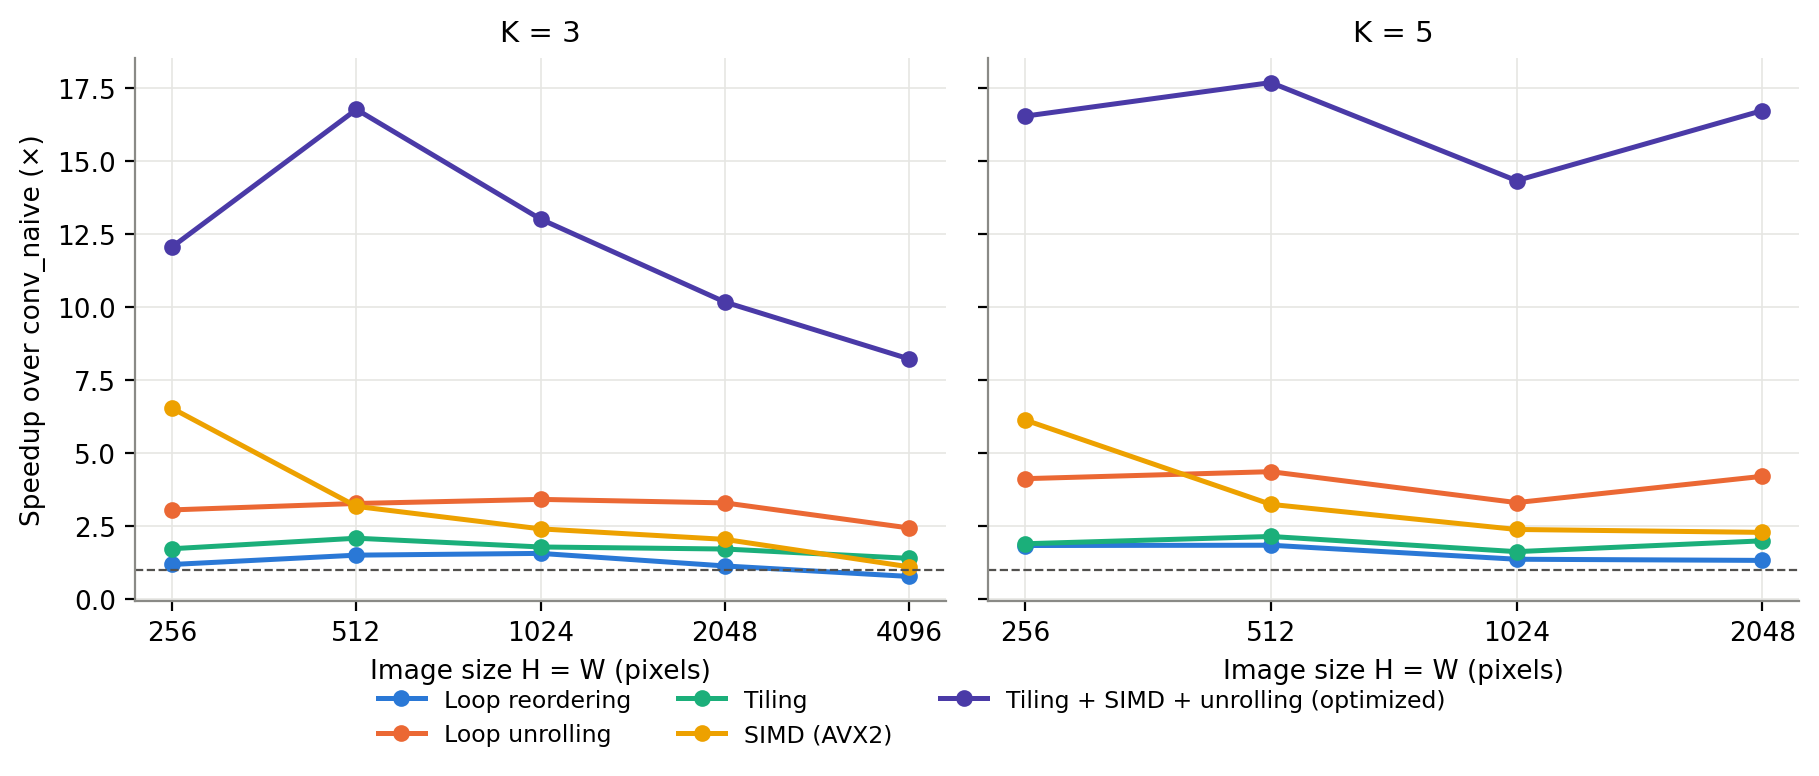
\includegraphics[width=\textwidth]{task1_speedup_vs_size.png}
\caption{Figure 1.1 equivalent: speedup over naive of each technique versus image size, $K=3$ (left) and $K=5$ (right). Data: \texttt{task1d\_sections234\_fixed.txt}.}
\label{fig:1d-size}
\end{figure}

\begin{figure}[H]
\centering
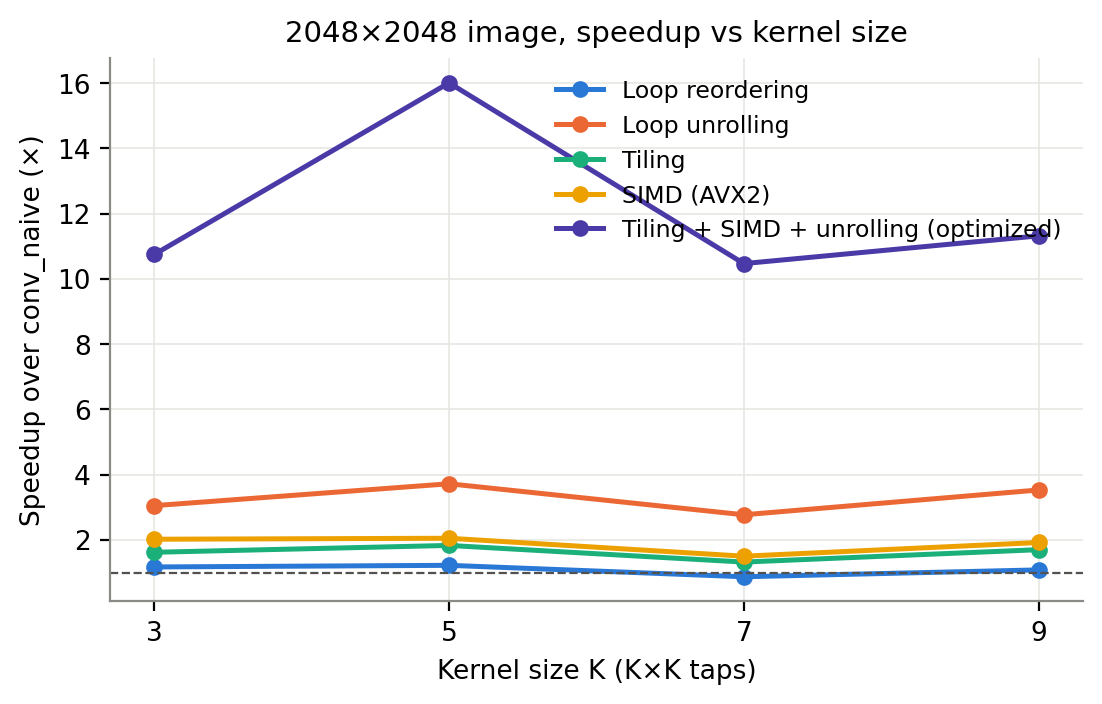
\includegraphics[width=0.62\textwidth]{task1_speedup_vs_kernel.png}
\caption{Speedup over naive versus kernel size at $2048\times2048$.}
\label{fig:1d-kernel}
\end{figure}

\subsection{Why the combination is more than the sum}

At $2048^2$, $K=3$ the best single techniques give 3.3$\times$ (unroll), 2.1$\times$ (SIMD) and 1.7$\times$ (tile). The combined kernel gives 10.2$\times$ in the same run and 9.25$\times$ in the graded run. That is more than the sum of the individual gains ($2.3+1.1+0.7 = 4.1$ on top of 1) and close to their product. Each technique removes a different limit, and each limit hides the next one.

SIMD on its own (1C) stops at about 2$\times$ because the reordered nest is memory-bound; the vector unit waits on the $K^2$ output read-modify-writes. Register accumulation removes those passes, but a scalar version of it (unroll, 1A) then runs into scalar FMA throughput at about 3$\times$. Putting SIMD on the register-accumulated form removes that compute limit, and the next one to appear is the re-reading of input rows; tiling keeps those rows in L1, and NACC=2 hides the FMA latency.

With all four in place the kernel runs at 36 to 73 GFLOP/s and is limited by the load ports, which is what the NACC sweep showed. Figures~\ref{fig:1d-size} and~\ref{fig:1d-kernel} show the combined kernel keeping an 8 to 17$\times$ margin at every size and kernel width, while every single technique slides towards 1$\times$ at 4096 as the image leaves L3. The fall from 16.8$\times$ at 512 to 8.2$\times$ at 4096 is DRAM bandwidth on the one unavoidable pass over input and output. At $K=5$ and $K=7$ there is more arithmetic per byte and the speedup rises to 16 to 17$\times$. The $K=7$ dip in Figure~\ref{fig:1d-kernel} comes from the naive baseline running unusually fast in that run (6.4 GFLOP/s against 4.5 to 5.1 elsewhere), not from the optimized kernel slowing down; it stays between 51 and 73 GFLOP/s.

\section{Summary}

Reordering gives 1 to 1.5$\times$ and unrolling about 3$\times$ (1A). Tiling (1B) removes the reorder's image-wide passes, holds 1.4 to 1.8$\times$, and cuts L1-D MPKI 7 to 17$\times$ against the untiled loop. We chose TH=4, TW=1024 because short, wide tiles avoid the power-of-two-stride set conflicts that make TH $\ge 16$ behave as if there were no tiling at all. SIMD (1C) cuts instructions 12.5$\times$ but buys only 1.1 to 2.5$\times$ because the un-tiled loop is bandwidth-bound. Combining register accumulation, AVX2 FMA, two independent accumulators and output tiling (1D) reaches 9.25$\times$ on the graded workload and 8 to 17$\times$ across sizes and kernel widths, more than the sum of the individual gains, because each technique removes the limit that stopped the previous one. We did not use software prefetching anywhere in Task 1, as required.

\end{document}
